\documentclass[tikz,border=10pt]{standalone}
\usetikzlibrary{positioning,arrows.meta,fit,backgrounds,shapes.geometric,calc}

\definecolor{coreindigo}{HTML}{3F51B5}
\definecolor{ifgreen}{HTML}{4CAF50}
\definecolor{fsgray}{HTML}{757575}

\begin{document}
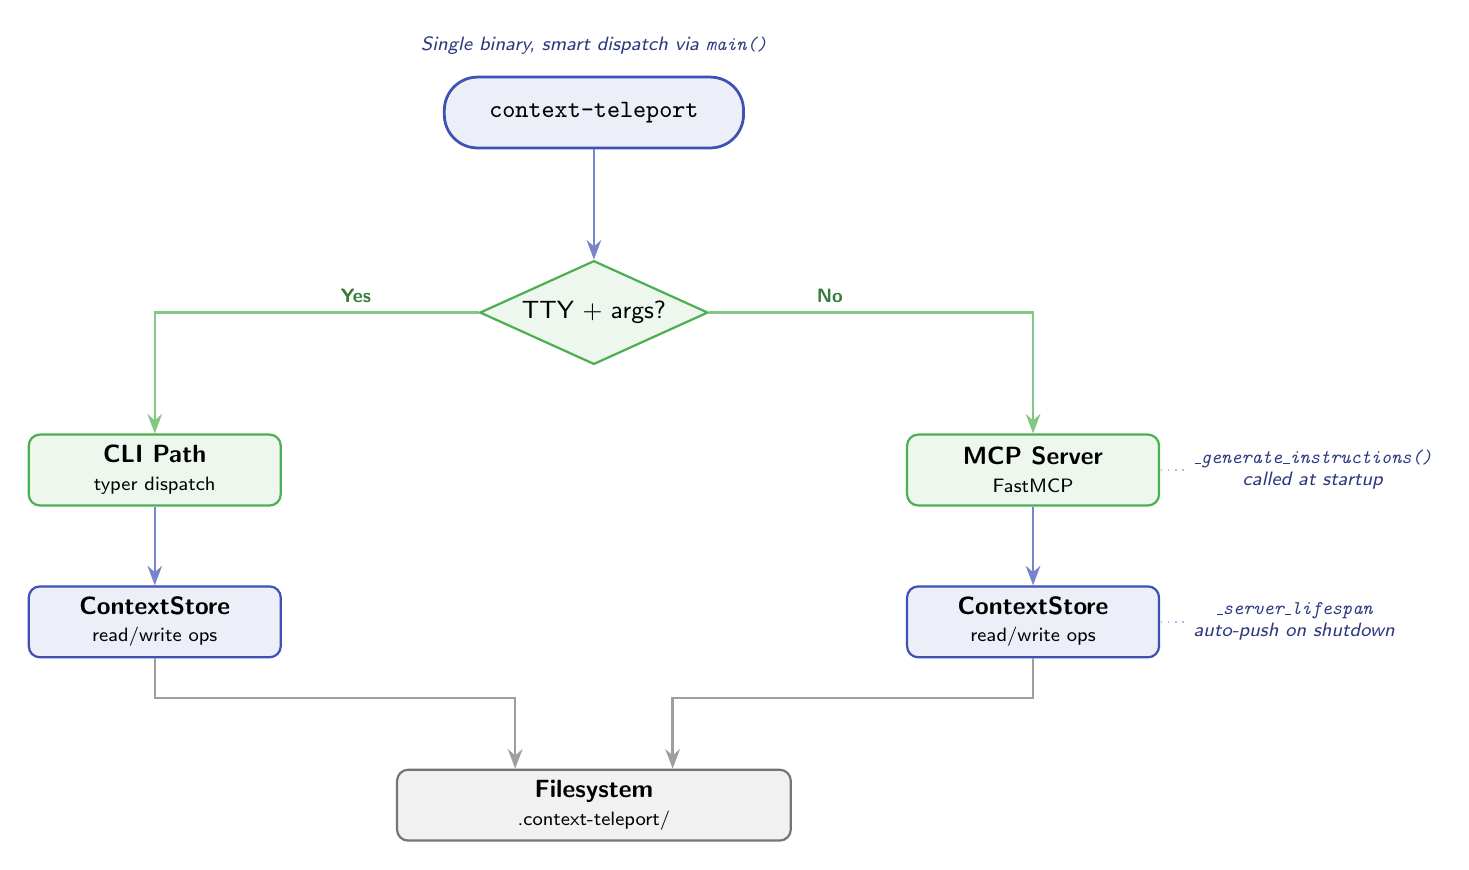
\begin{tikzpicture}[
    >=Stealth,
    every node/.style={font=\sffamily\small},
    proc/.style={
        draw=#1, fill=#1!10, rounded corners=4pt,
        minimum width=3.2cm, minimum height=0.9cm,
        line width=0.8pt, align=center
    },
    decision/.style={
        draw=#1, fill=#1!10, diamond, aspect=2.2,
        minimum width=2.4cm, inner sep=2pt,
        line width=0.8pt, font=\sffamily\small, align=center
    },
    start/.style={
        draw=#1, fill=#1!10, rounded corners=12pt,
        minimum width=3.8cm, minimum height=0.9cm,
        line width=1pt, font=\sffamily\small\bfseries
    },
    annot/.style={
        font=\sffamily\scriptsize\itshape, text=#1!70!black,
        align=center
    },
    arr/.style={->, thick, line width=0.9pt, color=#1!70},
]

% Start node
\node[start=coreindigo] (entry) {\texttt{context-teleport}};

% Decision diamond
\node[decision=ifgreen, below=1.4cm of entry] (decide) {TTY + args?};

% Arrow from start to decision
\draw[arr=coreindigo] (entry) -- (decide);

% === YES path: CLI ===
\node[proc=ifgreen, left=2.5cm of decide, yshift=-2cm] (cli) {\textbf{CLI Path}\\[-1pt]\scriptsize typer dispatch};
\node[proc=coreindigo, below=1cm of cli] (store1) {\textbf{ContextStore}\\[-1pt]\scriptsize read/write ops};

\draw[arr=ifgreen] (decide.west) -| node[above left, font=\sffamily\scriptsize\bfseries, text=ifgreen!70!black, pos=0.15] {Yes} (cli.north);
\draw[arr=coreindigo] (cli) -- (store1);

% === NO path: MCP ===
\node[proc=ifgreen, right=2.5cm of decide, yshift=-2cm] (mcp) {\textbf{MCP Server}\\[-1pt]\scriptsize FastMCP};
\node[proc=coreindigo, below=1cm of mcp] (store2) {\textbf{ContextStore}\\[-1pt]\scriptsize read/write ops};

\draw[arr=ifgreen] (decide.east) -| node[above right, font=\sffamily\scriptsize\bfseries, text=ifgreen!70!black, pos=0.15] {No} (mcp.north);
\draw[arr=coreindigo] (mcp) -- (store2);

% MCP annotations
\node[annot=coreindigo, right=0.3cm of mcp.east, anchor=west] (annot1)
    {\texttt{\_generate\_instructions()}\\called at startup};
\node[annot=coreindigo, right=0.3cm of store2.east, anchor=west] (annot2)
    {\texttt{\_server\_lifespan}\\auto-push on shutdown};

% Annotation lines
\draw[dotted, color=coreindigo!40, line width=0.6pt] (annot1.west) -- (mcp.east);
\draw[dotted, color=coreindigo!40, line width=0.6pt] (annot2.west) -- (store2.east);

% === Bottom: Filesystem (shared) ===
\node[proc=fsgray, minimum width=5cm, below=1.4cm of $(store1.south)!0.5!(store2.south)$] (fs)
    {\textbf{Filesystem}\\[-1pt]\scriptsize .context-teleport/};

\draw[arr=fsgray] (store1.south) -- ++(0,-0.5) -| ([xshift=-1cm]fs.north);
\draw[arr=fsgray] (store2.south) -- ++(0,-0.5) -| ([xshift=1cm]fs.north);

% Entry point annotation
\node[annot=coreindigo, above=0.15cm of entry.north, anchor=south]
    {Single binary, smart dispatch via \texttt{main()}};

\end{tikzpicture}
\end{document}
